\chapter{Results}

\section{Verification}

Test for each requirement.

\subsection{Time Resolution}

Test if smaller then \unit[1]{ms}.

\subsection{Spacial Resolution}

Inspect if smaller then \unit[1]{cm}. [physical size of sensor is 1 cm, sensor can be directly next to each other. show via drawing]

\subsection{Electrical Conductivity Resolution}

Test if able to distinguish liquids with a conductivity of \unitfrac[5]{S}{m} and \unitfrac[5e-3]{S}{m}.

\subsection{Cost}

Analyse if less than \euro{10} per sensor.

\subsection{Deployment}

Demonstrate that deployable in the algae reactor.

\subsection{Usability}

Test if easy to use by anybody with only a minimal set of written instructions. [find a victim to try to perform a measurement with only written instructions provided]

\section{Validation}

Check, if Timm can use it to measure flow and compare with simulation. [?]

\begin{figure}
	\begin{center}
		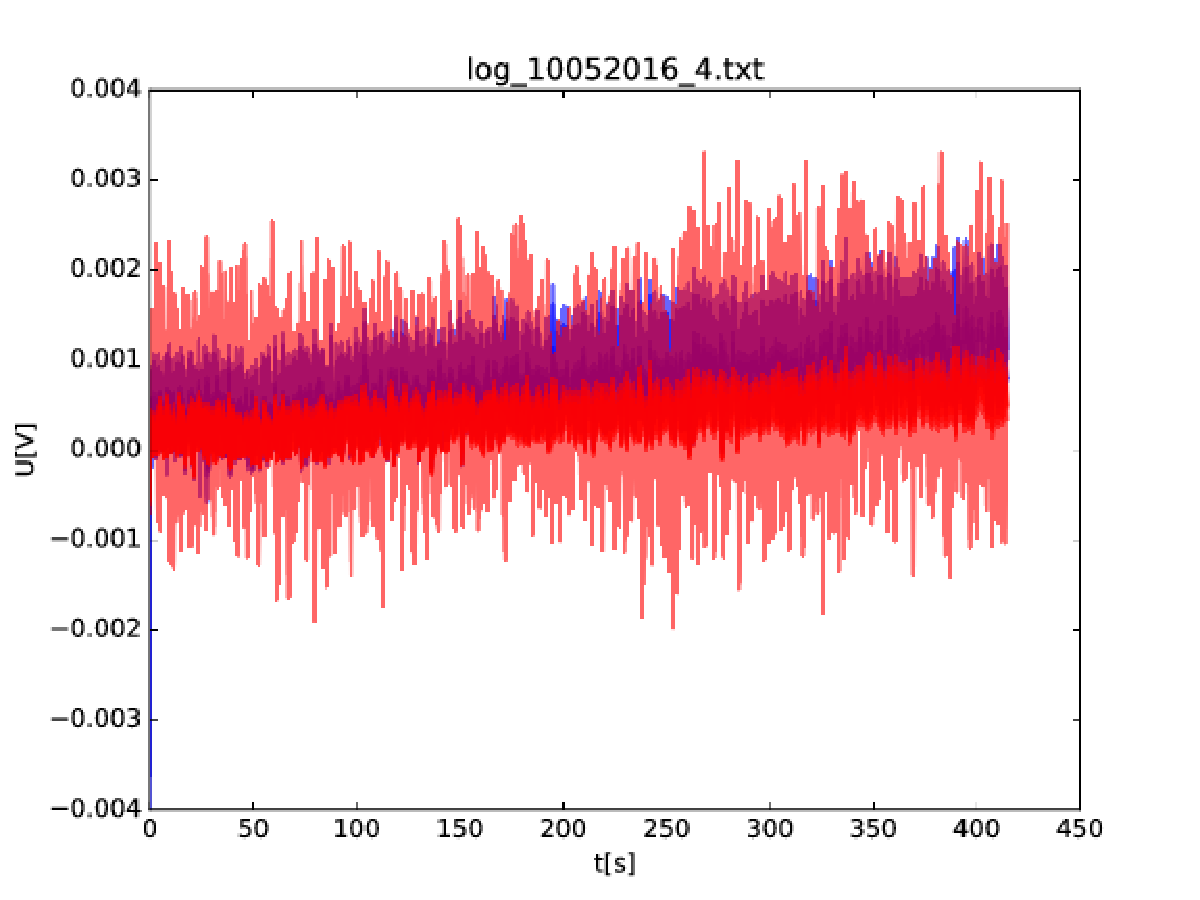
\includegraphics[width=\textwidth]{images/noise.pdf} 
		\caption{noise}
	\end{center}
\end{figure}

\begin{figure}
	\begin{center}
		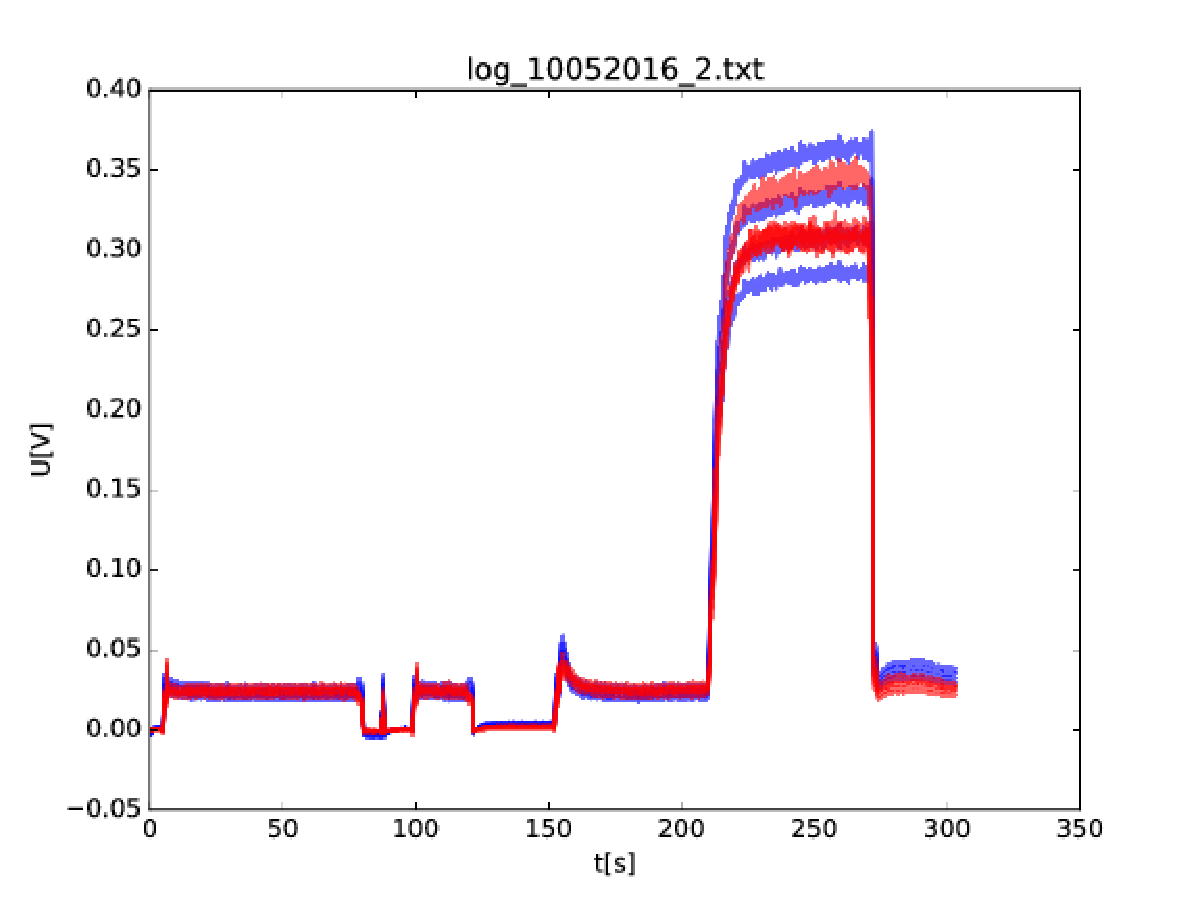
\includegraphics[width=\textwidth]{images/feed_switch.pdf} 
		\caption{feed switch}
	\end{center}
\end{figure}

\begin{figure}
	\begin{center}
		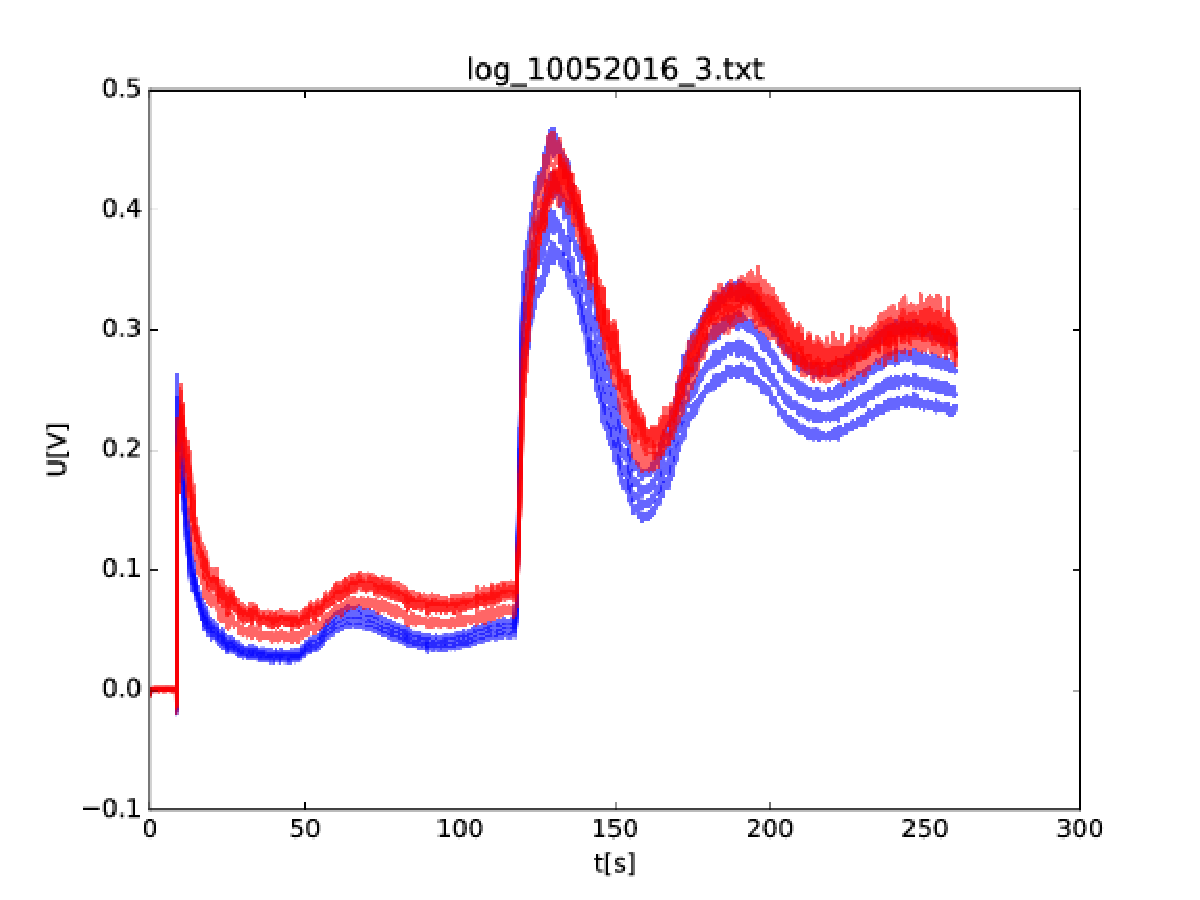
\includegraphics[width=\textwidth]{images/feed_add.pdf} 
		\caption{feed add}
	\end{center}
\end{figure}

\begin{figure}
	\begin{center}
		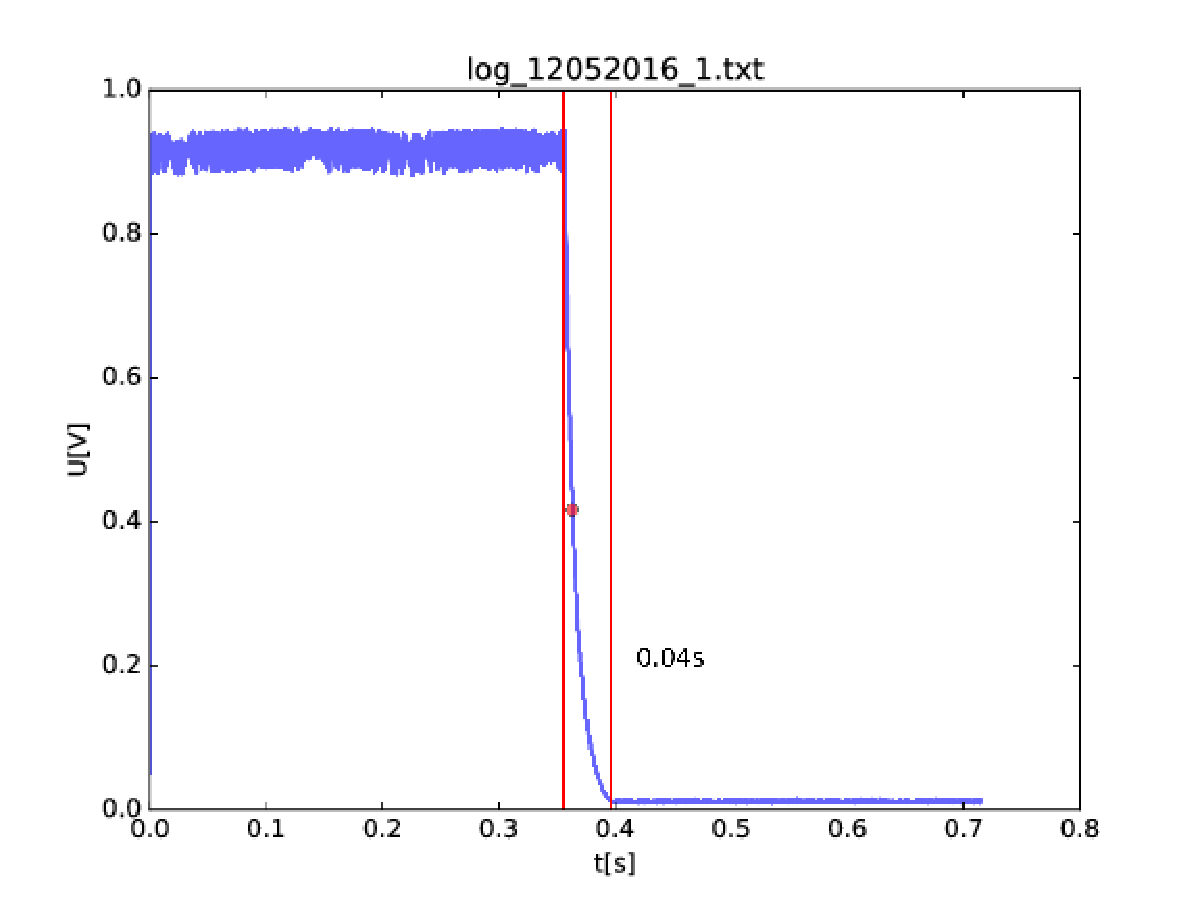
\includegraphics[width=\textwidth]{images/switch_cap.pdf} 
		\caption{switch cap}
	\end{center}
\end{figure}

\begin{figure}
	\begin{center}
		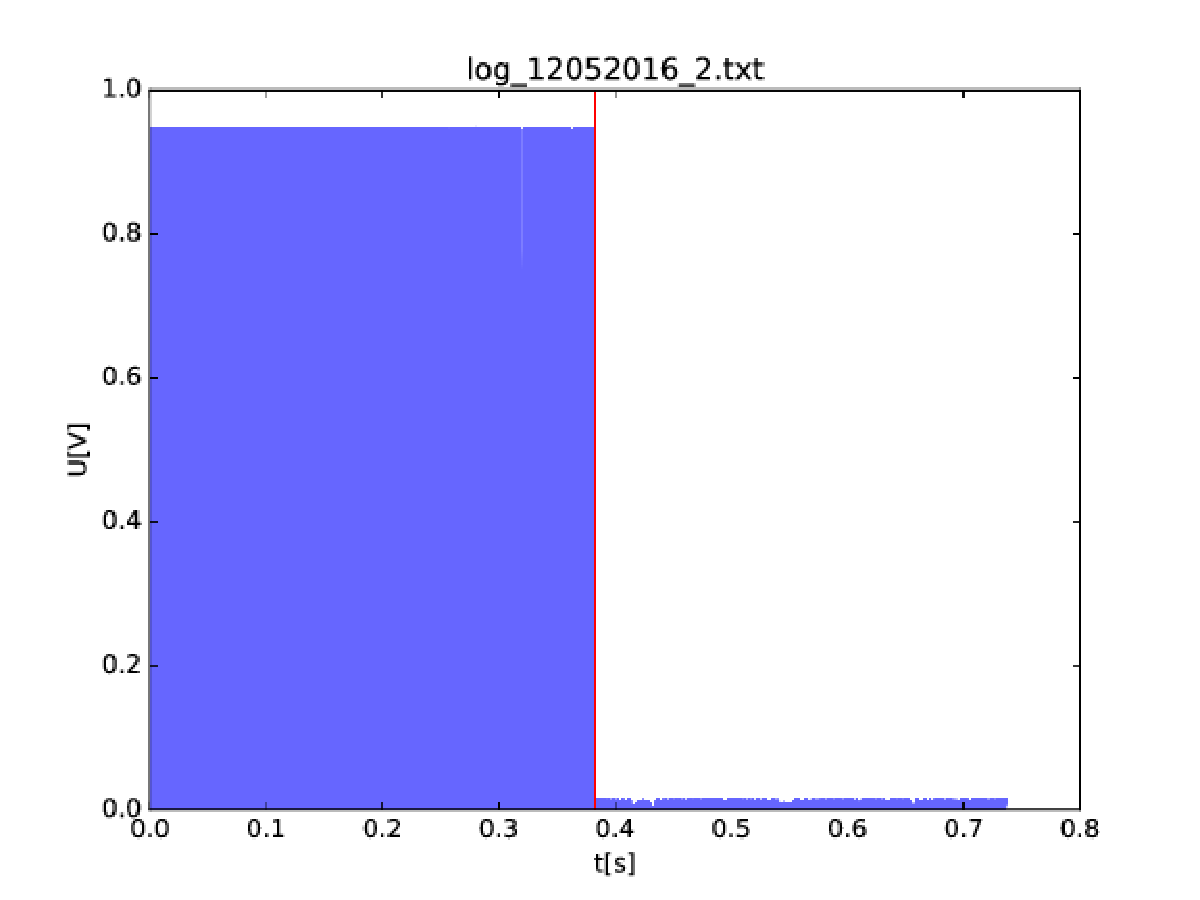
\includegraphics[width=\textwidth]{images/switch_nocap.pdf} 
		\caption{switch no cap}
	\end{center}
\end{figure}
